\documentclass[class=article, crop=false, dvipdfmx, fleqn]{standalone}
\title{航空機設計法第一 \\
レポート課題3 \ 機体三面図(初期案)}
\author{学籍番号 03-170313 飯山 敬大\\
        }
\date{\today}

% packages and libraries
\usepackage[utf8]{inputenc}				%fonts
\usepackage[ipaex]{pxchfon}
\usepackage{pifont}
\usepackage{mathtools, amssymb, mathrsfs, bbm,nccmath}	%math
\usepackage{siunitx, physics}
\usepackage[table]{xcolor}				%colors
\usepackage{tabularx}
\usepackage[dvipdfmx]{graphicx}					%figures
\usepackage{subcaption, wrapfig}
\usepackage{tikz}
\usetikzlibrary{calc, patterns, decorations, angles, calendar, backgrounds, shadows, mindmap}
\usepackage{tcolorbox}					%tables
\usepackage{longtable, float, multirow, array, listliketab, enumitem, tabularx}
\usepackage{listings}					%listings
\usepackage{comment}
\usepackage{hyperref}					%URL, link
\usepackage{url}
\usepackage{pxjahyper}
\usepackage{overcite}					%setting of citation
\usepackage{pxrubrica}					%rubi
\usepackage{fancyhdr, lastpage}			%pagelayout
\usepackage{import, grffile}			%file management
\usepackage{standalone}
\usepackage{bm}
\usepackage{empheq}
\usepackage{pdfpages}
\usepackage{multicol}
% set up for siunitx
\sisetup{%
	%detect-family = true,
	detect-inline-family = math,
	detect-weight = true,
	detect-inline-weight = math,
    %input-product = *,
    quotient-mode = fraction,
	fraction-function = \frac,
	inter-unit-product = \ensuremath{\hspace{-1.5pt}\cdot\hspace{-1.5pt}},
	per-mode = symbol,
	product-units = single,
	}

% setting of line skip
\setlength{\lineskiplimit}{6pt}
\setlength{\lineskip}{6pt}

% setting of indent
\setlength{\parindent}{1zw}
\setlength{\mathindent}{5zw}

% change cite form
\renewcommand{\citeform}[1]{[#1]}

% number equations only when they are referred to in the text
\mathtoolsset{showonlyrefs=true}
%\graphicspath{{images/}{../images/}}

% set up for hyperref
\hypersetup{%
	bookmarksnumbered = true,%
	hidelinks,%
	colorlinks = true,%
	linkcolor = black,%
	urlcolor = cyan,%
	citecolor = black,%
	filecolor = magenta,%
	setpagesize = false,%
	}

\pdfstringdefDisableCommands{%
\renewcommand*{\bm}[1]{#1}%
% any other necessary redefinitions
}
% Include \subsubsection in ToC
\setcounter{tocdepth}{3}

% tabularx
\newcolumntype{C}{>{\centering\arraybackslash}X} %セル内で中央揃え
\newcolumntype{R}{>{\raggedright\arraybackslash}X} %セル内で右揃え
\newcolumntype{L}{>{\raggedleft\arraybackslash}X}

\begin{document}
\section{概要}
  以下に示す設計要求を満たす航空機のサイジングを行う.なお,設計要求から, Blended Wing Body型
  として見積もりを行う.
  \begin{table}[H]
    \begin{center}
      \caption{設計要求}
      \begin{tabular}{l l} \hline
        Payload & 420Passengers(excluding 2 Pilots \& Cabin attendants) \\
        Range & 7500nm with max. payload,alternate airport(200nm) and \\
              & 45min. loiter \\
        Altitude & 38,000ft for the design Range \\
        Cruise Speed & M0.8 \\
        Climb & as required in FAR25. \\
        Take off \& landing & 10,000ft take-off field length at sea level \\
                 & 7000ft landing field length at $W_L=0.8W_{TO}$ at sea level \\
        Powerplants & Turbo Fan \\
        Certification Base & FAR25 \\
        Max. landing weight ratio & 0.88 \\  \hline
      \end{tabular}
    \end{center}
    \label{requirements}
  \end{table}

\section{設計点の変更}
前回行ったサイジングプロットでは, 設計点を$C_{L_{max}L} = 3.0, C_{L_{max}TO} = 2.2$の点
にとったが, 今回BWB機の胴体設計を行ったところ, この設計点では主翼が小さすぎて翼根部の厚さが足りず,
十分な客室高さを確保できないことが判明した. また, 無尾翼機として設計することに変更したため,
機体トリムの確保の問題から高性能の後縁フラップをつけることができず、
着陸時の$C_{L_{max}}$は通常の機体よりも小さな値になると考えられる. そこで下図のように設計点を左側に移し,
$C_{L_{max}L} = 1.9, C_{L_{max}TO} = 1.7$の両直線が交錯する場所とした. すると,
\begin{equation}
  \begin{cases}
    T = 2.44 \times 10^6 [Ib] \\
    S = 7.80 \times 10^3 [ft^2]
  \end{cases}
\end{equation}
となった. これを元に設計を進めていくことにする.

\begin{figure}[H]
  \begin{center}
  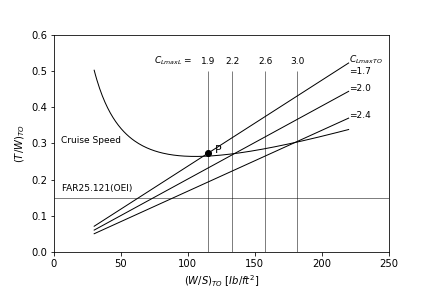
\includegraphics[width = 12cm]{../images/sizing.png}
  \caption{サイジングプロットの変更}
  \label{fig::sizing}
\end{center}
\end{figure}

\end{document}
